\documentclass[journal,10pt,twocolumn]{article}
\usepackage[margin=0.5in]{geometry}
\usepackage[cmex10]{amsmath}
\usepackage{array}
\usepackage{booktabs}
% The preceding line is only needed to identify funding in the first footnote. If that is unneeded, please comment it out.
\usepackage{cite}
\usepackage{amsmath,amssymb,amsfonts}
\usepackage{graphicx}
\usepackage{textcomp}
\usepackage{xcolor}
\usepackage{graphicx}
\graphicspath{{./fig}}{}
\def\BibTeX{{\rm B\kern-.05em{\sc i\kern-.025em b}\kern-.08em
    T\kern-.1667em\lower.7ex\hbox{E}\kern-.125emX}}
\usepackage{tikz}
\usetikzlibrary{shapes.geometric}
\usetikzlibrary{shapes.geometric,angles,quotes}
\begin{document}
\newtheorem{theorem}{Theorem}[section]
\newtheorem{problem}{Problem}
\newtheorem{proposition}{Proposition}[section]
\newtheorem{lemma}{Lemma}[section]
\newtheorem{corollary}[theorem]{Corollary}
\newtheorem{example}{Example}[section]
\newtheorem{definition}[problem]{Definition}
%\newtheorem{thm}{Theorem}[section] 
%\newtheorem{defn}[thm]{Definition}
%\newtheorem{algorithm}{Algorithm}[section]
%\newtheorem{cor}{Corollary}
\newcommand{\BEQA}{\begin{eqnarray}}
\newcommand{\EEQA}{\end{eqnarray}}
\newcommand{\define}{\stackrel{\triangle}{=}}
\newcommand*\circled[1]{\tikz[baseline=(char.base)]{
    \node[shape=circle,draw,inner sep=2pt] (char) {#1};}}
\bibliographystyle{article}
%\bibliographystyle{ieeetr}
\providecommand{\mbf}{\mathbf}
\providecommand{\pr}[1]{\ensuremath{\Pr\left(#1\right)}}
\providecommand{\re}[1]{\ensuremath{\text{Re}\left(#1\right)}}
\providecommand{\im}[1]{\ensuremath{\text{Im}\left(#1\right)}}
\providecommand{\qfunc}[1]{\ensuremath{Q\left(#1\right)}}
\providecommand{\sbrak}[1]{\ensuremath{{}\left[#1\right]}}
\providecommand{\lsbrak}[1]{\ensuremath{{}\left[#1\right.}}
\providecommand{\rsbrak}[1]{\ensuremath{{}\left.#1\right]}}
\providecommand{\brak}[1]{\ensuremath{\left(#1\right)}}
\providecommand{\lbrak}[1]{\ensuremath{\left(#1\right.}}
\providecommand{\rbrak}[1]{\ensuremath{\left.#1\right)}}
\providecommand{\cbrak}[1]{\ensuremath{\left\{#1\right\}}}
\providecommand{\lcbrak}[1]{\ensuremath{\left\{#1\right.}}
\providecommand{\rcbrak}[1]{\ensuremath{\left.#1\right\}}}
\newcommand{\sgn}{\mathop{\mathrm{sgn}}}
%\providecommand{\hilbert}{\overset{\mathcal{H}}{ \rightleftharpoons}}
\providecommand{\system}{\overset{\mathcal{H}}{ \longleftrightarrow}}
	%\newcommand{\solution}[2]{\textbf{Solution:}{#1}}
\newcommand{\solution}{\noindent \textbf{Solution: }}
\newcommand{\cosec}{\,\text{cosec}\,}
\providecommand{\dec}[2]{\ensuremath{\overset{#1}{\underset{#2}{\gtrless}}}}
\newcommand{\myvec}[1]{\ensuremath{\begin{pmatrix}#1\end{pmatrix}}}
\newcommand{\mydet}[1]{\ensuremath{\begin{vmatrix}#1\end{vmatrix}}}
	\newcommand*{\permcomb}[4][0mu]{{{}^{#3}\mkern#1#2_{#4}}}
\newcommand*{\perm}[1][-3mu]{\permcomb[#1]{P}}
\newcommand*{\comb}[1][-1mu]{\permcomb[#1]{C}}
%\numberwithin{equation}{section}
\numberwithin{equation}{subsection}
%\numberwithin{problem}{section}
%\numberwithin{definition}{section}
\let\vec\mathbf
\title{
{Deriving the equation of Circle with given Area and Center \\
which is crossing point of two diameter lines\\
Using Matrices}\\
\author{T.ManasaReddy}
\maketitle
\tableofcontents
\section{Problem}
The lines 3x-4y=7 and 2x-3y=5 are diameters of a circle having area 49 $\pi$ Then find the equation of Circle.
\section{Considerations}
\vspace{0.2cm}
The input parameters are the lengths r, c and angle $\theta$. \\
\vspace{0.2cm}
{
\setlength\extrarowheight{2pt}
\begin{tabular}{|c|c|c|}
	\hline
	\textbf{Symbol}&\textbf{Value}&\textbf{Description}\\
	\hline
	$\vec{O}$ & \myvec{0\\0}
	&Origin\\
	\hline
	r&  & Radius of the Circle\\
	\hline
	$\vec{C}$ & \myvec{x \\ y}
	&Center of the Circle
	\\
\hline
\end{tabular}
}
\section{Plotting the Circle with center and radius}
\vspace{0.25cm}
Plot of the Circle with center $\vec{C} =\myvec{1\\-1}$ and radius r=7  is shown in figure 1, where the point C is the crossing point of the given diameter lines, 2x-3y=5 and 3x-4y=7.
\begin{figure}[h]
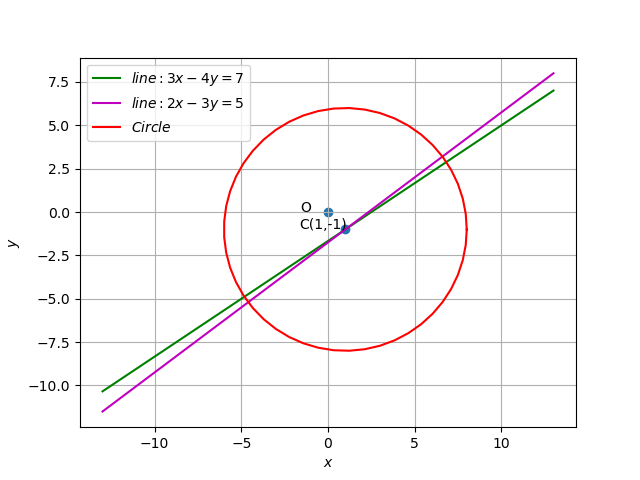
\includegraphics[width=1\columnwidth]{circle.png}
\caption{Circle with radius r=7 and center C(1, -1)}
\label{fig:Circle with radius and center}
\end{figure}
\section{Solution}
\vspace{0.25cm}
\subsection{Finding the center C of the Circle}
\begin{flushleft}
Let O be the origin and its coordinates are\\
\vspace{0.25cm}
\begin{center}
$\vec{O} = \myvec{0\\0}$ 
\end{center}
Given line equations are
\begin{equation}
2x-3y = 5  
\end{equation}
\begin{equation}
3x-4y = 7  
\end{equation}
The above equations can be written in matrix form as,
\center
\myvec{ 2 & -3 \\ 3 & -4} \myvec{x \\ y} = \myvec{5\\7} \\
\vspace\center
\myvec{ 2 & -3 \\ 3 & -4} \myvec{x \\ y} = \myvec{5\\7} \\
\vspace{0.3cm}
\begin{flushleft}
The augmented matrix can be expressed as,
\end{flushleft}
\myvec{ \circled{2} & -3 & 5 \\ 3 & -4 & 7} \\
\begin{flushleft}
Through pivoting, the augmented matrix will become as,
\end{flushleft}
\myvec{ 1 & 0 & 1 \\ 0 & 1 & -1} \{0.3cm}
\begin{flushleft}
The augmented matrix can be expressed as,
\end{flushleft}
\myvec{ \circled{2} & -3 & 5 \\ 3 & -4 & 7} \\
\begin{flushleft}
Through pivoting, the augmented matrix will become as,
\end{flushleft}
\myvec{ 1 & 0 & 1 \\ 0 & 1 & -1} \\\center
\myvec{ 2 & -3 \\ 3 & -4} \myvec{x \\ y} = \myvec{5\\7} \\
\vspace{0.3cm}
\begin{flushleft}
The augmented matrix can be expressed as,
\end{flushleft}
\myvec{ \circled{2} & -3 & 5 \\ 3 & -4 & 7} \\
\begin{flushleft}
Through pivoting, the augmented matrix will become as,
\end{flushleft}
\myvec{ 1 & 0 & 1 \\ 0 & 1 & -1} \
\begin{flushleft}
On solving above equation the crossing point of the given equations will be,\\
\end{flushleft}
\myvec{x\\y}= \myvec{1\\-1}
\endcenter
\begin{flushleft}
Therefore the Center of the Circle is,\\
\end{flushleft}
\begin{equation}
    \vec{C} = \myvec{1\\-1}
\end{equation}
\end{flushleft}
\subsection{Calculation of radius of the Circle}
As per the given data, the area of the Circle is 154 sq.units\\
Let r be the radius of circle,\\
\begin{equation}
\pi r^2 = 154 \implies r = 7
\end{equation}
\subsection{Deriving equation for Circle in matrix form}
\vspace{0.2cm}
\begin{flushleft}
The equation of circle in matrix form is,\\
\vspace{0.25cm}
\end{flushleft}
\vspace{0.25cm}
\begin{equation}
 \vec{x}^T \vec{V} \vec{x} + 2 \vec{u}^T \vec{x} + f = 0
\end{equation}
\begin{flushleft}
Where\\
\end{flushleft}
\center
$\vec{V} = \vec{I}= \myvec{ 1 & 0\\ 0 & 1} , \vec{u} = \myvec{-1 \\ 1}, \vec{f}=-47$\\
\endcenter
\center
  $\implies$  $ \vec{x}^T$$\vec{I}$ $\vec{x}$  + 2 $ \myvec{-1\\1}^T \vec{x} -47 = 0$
\endcenter
\begin{flushleft}
\vspace{0.23cm}
Therefore, the circle equation can be written as
\end{flushleft}
\begin{equation}
    \vec{x}^T \vec{x} + 2 \myvec{-1\\1}^T \vec{x} -47 = 0
\end{equation}
\endcenter
\begin{flushleft}
\vspace{0.2cm}
\subsection{Deriving equation for Circle in quadratic form}
In quadratic form, the expression for circle  can be written as,
\end{flushleft}
\center
  $$  (x-x1)^2+(y-y1)^2 = r^2 $$\\
    $$(x-1)^2+(y+1)^2 = 7^2$$
\endcenter
\begin{equation}
    x^2+y^2-2x+2y-47=0
\end{equation}
\section{Conclusion}
\begin{flushleft}
1. At first, Center of the Circle has been found which is crossing point of the two diameter lines 2x-3y=5 and 3x-4y=7.\\
\vspace{0.25cm}
2. Radius of the center has been calculated from its area 154sq.units.\\
\vspace{0.25cm}
3. Matrix equation for $\vec{V, U, U^T}$ and $\vec{f}$ has been derived.\\
\vspace{0.25cm}
4. Finally, the Circle equation has been derived as, \\
\vspace{0.25cm}
\begin{center}
$  \vec{x}. \vec{x}^T + 2 \myvec{-1\\1}^T \vec{x} -47 = 0$
\end{center}
\end{flushleft}
\end{document}
